\chapter{Diagramas de Penrose y formación de un agujero negro real}

La representación de Kruskal ofrece una descripción elegante de las proximidades del horizonte de Schwarzschild, pero un agujero negro real no es eterno: se forma cuando colapsa la materia. ¿Qué partes de la representación extendida sobreviven a esa historia física? Para responder, necesitamos un diagrama lo bastante grande como para contener un espaciotiempo entero y lo bastante disciplinado como para conservar el movimiento de la luz. Primero compactificaremos el espaciotiempo plano, luego el espaciotiempo de Schwarzschild y, por último, uniremos las partes adecuadas a través de una capa de radiación que cae hacia dentro.

\section{Cerca del horizonte: repaso de Kruskal y los cuatro cuadrantes}

Empezamos exactamente donde terminó la clase anterior. Muy cerca del horizonte de Schwarzschild, la geometría se parece localmente a la del espacio plano. El propio horizonte se comporta como el lugar geométrico de unas coordenadas polares hiperbólicas, de manera parecida a lo que ocurre con las coordenadas aceleradas en el espaciotiempo ordinario de Minkowski. En esta representación local imponemos desde el principio una regla que nunca abandonaremos: los rayos de luz radiales se dibujan a \(45^\circ\), y toda línea de universo temporal debe ser más inclinada que esas líneas nulas.

Conviene interpretar las coordenadas de este repaso como el tiempo y el espacio tal como los ve un observador en caída libre. En esas coordenadas localmente inerciales, las proximidades del horizonte parecen casi planas. Pero un observador que insiste en mantenerse suspendido a radio fijo fuera del agujero no es inercial. Respecto del sistema de referencia en caída libre, esa persona sigue una curva acelerada. Cuanto más cerca se mantiene del horizonte, mayor es la aceleración necesaria para no caer. Ese es el significado físico de la familia de curvas exteriores dibujada en el lado derecho de la pizarra.

\begin{figure}[htbp]
\centering
\includegraphics[width=0.72\textwidth]{lecture_08_figure_02.png}
\caption{Esquema en la pizarra de la geometría de cuatro regiones cerca del horizonte. Las curvas rojas del exterior representan una familia de líneas de universo de observadores suspendidos a radio fijo.}
\lectureframe{00:02:54}
\end{figure}

\begin{figure}[htbp]
\centering
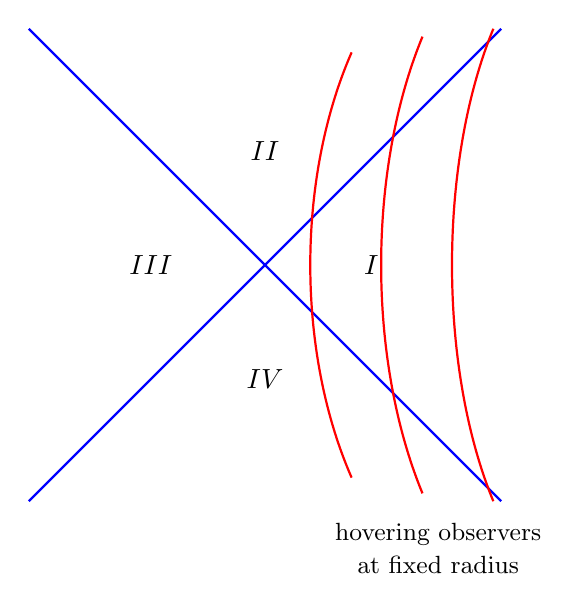
\begin{tikzpicture}[scale=1.0]
\draw[thick,blue] (-3,3) -- (3,-3);
\draw[thick,blue] (-3,-3) -- (3,3);

\draw[red,thick] (1.1,-2.7) .. controls (0.4,-1.1) and (0.4,1.1) .. (1.1,2.7);
\draw[red,thick] (2.0,-2.9) .. controls (1.3,-1.2) and (1.3,1.2) .. (2.0,2.9);
\draw[red,thick] (2.9,-3.0) .. controls (2.2,-1.3) and (2.2,1.3) .. (2.9,3.0);

\node at (1.35,0.0) {$I$};
\node at (0.0,1.45) {$II$};
\node at (-1.45,0.0) {$III$};
\node at (0.0,-1.45) {$IV$};

\node[align=center] at (2.2,-3.6) {\small hovering observers\\\small at fixed radius};
\end{tikzpicture}
\caption{Redibujo limpio de la estructura causal de tipo Kruskal empleada en el repaso. La región \(I\) es el exterior, la región \(II\) es el interior ineludible, y las regiones \(III\) y \(IV\) pertenecen a la extensión formal que más adelante descartaremos para describir un agujero negro real formado por colapso.}
\end{figure}

Esto basta para describir lo que hace un agujero negro. En la región exterior \(I\), los objetos y las señales pueden dirigirse hacia dentro, pero también pueden permanecer fuera o volver a salir. En cambio, en la región \(II\), el destino causal está determinado. Una vez dentro, no hay ningún camino causal dirigido hacia el futuro que lleve de vuelta al exterior. Para escapar de la región \(II\) hacia cualquiera de las regiones exteriores habría que seguir, en algún punto, una trayectoria menos inclinada que \(45^\circ\) y, por tanto, más rápida que la luz. Toda trayectoria temporal futura permitida termina en la singularidad.

Este repaso inicial no es una mera repetición. Prepara el tema central del capítulo. La representación de Kruskal es útil, pero no todas sus partes tienen significado físico para un agujero negro real.

\begin{classroomqa}
\audiencequestion{¿Cuáles son los ejes del diagrama y de quiénes son las líneas de universo de posición fija representadas por las curvas rojas?}
\lecturerresponse{Los ejes representan el tiempo y el espacio en coordenadas naturales para un observador en caída libre. Cerca del horizonte, ese observador ve un espaciotiempo casi plano y ordinario. En cambio, las curvas rojas de posición constante corresponden a observadores que se mantienen estacionarios fuera del agujero. Sus líneas de universo son aceleradas, y la aceleración necesaria aumenta al acercarse al horizonte.
\lecturetimestamp{00:05:58--00:06:47}}
\end{classroomqa}

\section{¿Por qué compactificar? Del espaciotiempo infinito a una pizarra finita}

El siguiente paso es metodológico. Las direcciones nulas de estos diagramas se prolongan hasta el infinito, y el tiempo también. Por eso no podemos dibujar todo el espaciotiempo en una pizarra corriente sin cambiar de coordenadas. La motivación del profesor es muy concreta: si queremos verlo todo a la vez y razonar sobre la estructura causal global, necesitamos una manera de comprimir un espaciotiempo infinito en una región finita sin dejar de reconocer los rayos de luz.

Así que vuelve al caso sencillo, el buen y viejo espaciotiempo plano. Como los problemas que nos interesan tienen simetría esférica, suprimimos las direcciones angulares y conservamos solo el tiempo y la coordenada radial. Usamos las coordenadas \(T\) y \(R\), con
\[
R\ge 0,
\]
ya que una distancia radial negativa no tiene sentido en coordenadas polares. También elegimos unidades en las que
\[
c=1.
\]
Con esta convención, el movimiento radial nulo se dibuja a \(45^\circ\).

Antes de introducir la transformación de compactificación, la clase se detiene un momento para orientarnos en el plano \(T\)-\(R\). Se dibuja el eje temporal, el eje radial, algunas secciones de tiempo constante \(T=0,\pm1,\pm2\) y algunas líneas de radio constante \(R=1,2,3\). No se trata de formalismo vacío. Nos proporciona puntos de referencia y deja claro qué rasgos queremos conservar cuando luego comprimamos el diagrama hasta darle un tamaño finito.

También hay un detalle pedagógico sutil, pero importante, sobre el origen. En la representación radial reducida, un rayo de luz dirigido exactamente hacia \(R=0\) parece rebotar en el origen y volver hacia fuera. Pero no hay nada que rebote físicamente contra una pared. En la geometría completa con simetría esférica, el rayo simplemente atraviesa el origen y emerge por el otro lado. El rebote aparente es solo consecuencia de trabajar con el semiplano \(R\ge 0\).

De manera similar, un rayo de luz que no pasa por el origen empieza pareciendo casi igual, llega a un punto de máxima aproximación y luego se curva hacia fuera. En estas coordenadas, incluso puede parecer que algo lo ha repelido desde el origen. Pero también eso es una descripción en coordenadas de la conocida barrera del momento angular, no una fuerza nueva. El profesor se detiene en estos ejemplos porque quiere que el público confíe en el diagrama antes de deformarlo.

Ahora viene el paso esencial. Vamos a comprimir y estirar la representación, pero mantendremos fijo un rasgo: los rayos de luz radiales deben seguir siendo líneas a \(45^\circ\). Ese es el propósito de la compactificación.

\begin{classroomqa}
\audiencequestion{¿Hay algo físicamente especial en el origen elegido? ¿Los rayos aparentemente curvados indican que allí actúa una fuerza?}
\lecturerresponse{No. En esta etapa, el origen es simplemente el centro que seleccionan las coordenadas esféricas. El rebote y la curvatura aparentes se deben a que reducimos el movimiento espacial completo a \(R\geq0\). La simetría puede hacer conveniente elegir un centro, como sucede con el Sol, pero la elección de coordenadas no coloca allí un agujero negro ni una pared reflectante.
\lecturetimestamp{00:16:27--00:17:08}}
\end{classroomqa}

\section{Espaciotiempo plano en coordenadas nulas y forma de Penrose}

Para precisar la deformación, introducimos coordenadas nulas. Esta es la parte matemáticamente limpia de la clase, y el profesor muestra explícitamente el paso en la pizarra.

\begin{figure}[htbp]
\centering
\includegraphics[width=0.82\textwidth]{lecture_08_figure_03.png}
\caption{La pizarra despejada con los ejes \(T\)-\(R\), al introducir \(T^+=T+R\) y \(T^-=T-R\). El origen radial reducido es la línea vertical azul \(R=0\).}
\lectureframe{00:19:45}
\end{figure}

Definimos
\begin{align}
T^+ &= T+R, \\
T^- &= T-R.
\end{align}
Estas coordenadas se adaptan al movimiento nulo radial. Un rayo de luz radial entrante tiene \(T^+=\text{const}\), mientras que uno saliente tiene \(T^-=\text{const}\).

\paragraph{Derivación.}
En estas coordenadas, la línea \(R=0\) se expresa de forma particularmente sencilla. En efecto,
\begin{align}
R=0
&\iff T+R=T-R \\
&\iff T^+=T^-.
\end{align}
Así, toda la frontera temporal \(R=0\) queda descrita mediante una sola relación:
\begin{equation}
R=0 \iff T^+=T^-.
\end{equation}

\begin{figure}[htbp]
\centering
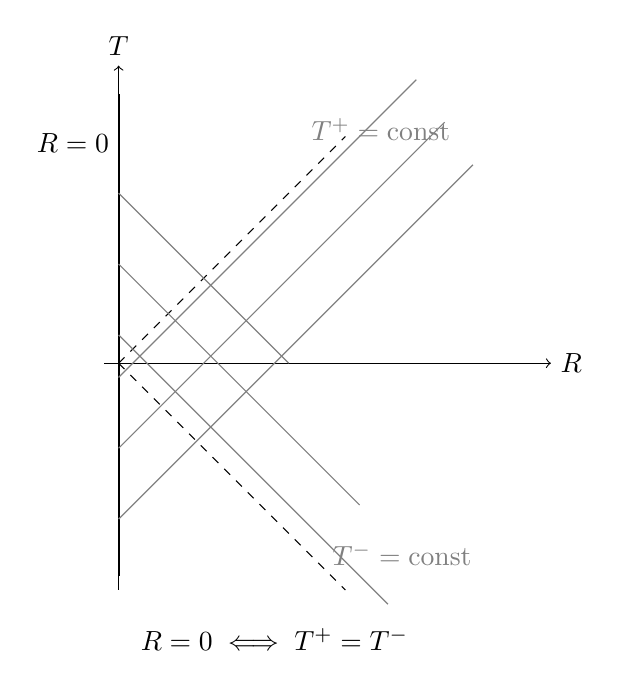
\begin{tikzpicture}[scale=0.9]
\draw[->] (-0.2,0) -- (6.1,0) node[right] {$R$};
\draw[->] (0,-3.2) -- (0,4.2) node[above] {$T$};

\draw[thick] (0,-3.0) -- (0,3.8);
\node[left] at (0,3.1) {$R=0$};

\draw[dashed] (0,0) -- (3.2,3.2);
\draw[dashed] (0,0) -- (3.2,-3.2);

\draw[gray] (0,2.4) -- (2.4,0);
\draw[gray] (0,1.4) -- (3.4,-2.0);
\draw[gray] (0,0.4) -- (3.8,-3.4);

\draw[gray] (0,-2.2) -- (5.0,2.8);
\draw[gray] (0,-1.2) -- (4.6,3.4);
\draw[gray] (0,-0.2) -- (4.2,4.0);

\node[gray] at (3.7,3.3) {$T^+=\mathrm{const}$};
\node[gray] at (4.0,-2.7) {$T^-=\mathrm{const}$};

\node at (2.2,-3.9) {$R=0 \iff T^+=T^-$};
\end{tikzpicture}
\caption{Redibujo limpio en coordenadas \(T\)-\(R\). Las dos familias nulas son las curvas de nivel de \(T^+\) y \(T^-\), y la línea \(R=0\) se expresa de forma equivalente como \(T^+=T^-\).}
\end{figure}

Ahora compactificamos. Introducimos dos nuevas coordenadas nulas, \(U^\pm\), cada una obtenida a partir de la correspondiente \(T^\pm\) mediante la misma función monótona y acotada \(F\):
\begin{align}
U^+ &= F(T^+), &
U^- &= F(T^-),
\end{align}
con
\begin{equation}
F(+\infty)=1,
\qquad
F(-\infty)=-1.
\end{equation}
La elección práctica de la clase es
\begin{equation}
F(x)=\tanh x,
\end{equation}
con lo que
\begin{equation}
U^+ = \tanh(T^+),
\qquad
U^- = \tanh(T^-).
\end{equation}
La tangente hiperbólica no tiene nada de especial. Es simplemente una función suave con el comportamiento límite adecuado y, por tanto, comprime intervalos coordenados infinitos hasta hacerlos finitos.

La estructura nula se conserva por una razón sencilla. Si un rayo de luz radial entrante tiene \(T^+=\text{const}\), entonces
\[
U^+=F(T^+)=\text{const},
\]
y, de forma análoga, si un rayo de luz radial saliente tiene \(T^-=\text{const}\), entonces
\[
U^-=F(T^-)=\text{const}.
\]
Así, la compactificación cambia por separado la parametrización de las dos direcciones nulas, y los rayos de luz radiales siguen siendo líneas a \(45^\circ\). La línea del origen se transforma con la misma sencillez:
\[
T^+=T^- \Longrightarrow U^+=U^-.
\]

En este punto, el semiplano infinito del espaciotiempo plano se ha comprimido hasta formar un triángulo finito. A continuación, la clase nos enseña a interpretar sus bordes. El infinito espacial se contrae hasta un único punto \(i^0\). Los infinitos temporales futuro y pasado son \(i^+\) y \(i^-\). Los dos bordes nulos son \(\mathcal{I}^+\) y \(\mathcal{I}^-\), que suelen pronunciarse «scri plus» y «scri minus»; son los lugares donde empiezan y terminan los rayos de luz entrantes y salientes.

\begin{figure}[htbp]
\centering
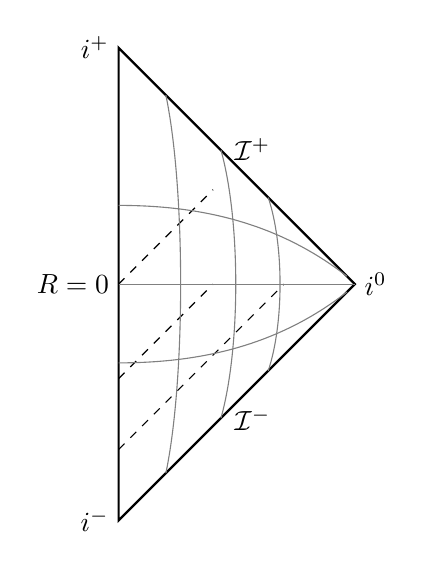
\begin{tikzpicture}[scale=1.0]
\draw[thick] (0,-3) -- (0,3) -- (3,0) -- cycle;

\node[left] at (0,3) {$i^+$};
\node[left] at (0,-3) {$i^-$};
\node[right] at (3,0) {$i^0$};
\node[left] at (0,0) {$R=0$};
\node[above right] at (1.35,1.45) {$\mathcal{I}^+$};
\node[below right] at (1.35,-1.45) {$\mathcal{I}^-$};

\draw[dashed] (0,-2.1) -- (2.1,0.0);
\draw[dashed] (0,-1.2) -- (1.2,0.0);
\draw[dashed] (0,0.0) -- (1.2,1.2);

\draw[gray] (0,0) -- (3,0);
\draw[gray] (0,1.0) .. controls (1.0,1.0) and (2.0,0.8) .. (2.9,0.1);
\draw[gray] (0,-1.0) .. controls (1.0,-1.0) and (2.0,-0.8) .. (2.9,-0.1);

\draw[gray] (0.6,-2.4) .. controls (0.85,-1.2) and (0.85,1.2) .. (0.6,2.4);
\draw[gray] (1.3,-1.7) .. controls (1.55,-0.8) and (1.55,0.8) .. (1.3,1.7);
\draw[gray] (1.9,-1.1) .. controls (2.1,-0.5) and (2.1,0.5) .. (1.9,1.1);
\end{tikzpicture}
\caption{Diagrama de Penrose del espaciotiempo plano con simetría radial reducida. Las curvas de tiempo constante se extienden hacia \(i^0\), mientras que las curvas de radio constante ascienden desde \(i^-\) hacia \(i^+\).}
\end{figure}

Conviene recordar un último punto de la clase. Estos diagramas \emph{no} conservan las distancias métricas. Conservan la estructura causal. Eso es lo que buscamos que permanezca invariante.

\begin{classroomqa}
\audiencequestion{¿Se supone que las líneas compactificadas de tiempo constante son rectas?}
\lecturerresponse{Solo la sección simétrica \(T=0\) es recta para la transformación elegida. Las otras curvas de tiempo constante \(T\) se curvan, y su forma detallada depende de la función de compactificación. Las secciones muy tardías se apiñan cada vez más cerca del borde superior, aunque el tiempo ordinario siga transcurriendo sin límite.
\lecturetimestamp{00:29:11--00:30:12}}
\end{classroomqa}

\section{La geometría de Schwarzschild compactificada}

Con la construcción del espacio plano ya establecida, volvemos ahora al agujero negro y repetimos el procedimiento. Compactificamos la geometría de Kruskal introduciendo coordenadas nulas y comprimiendo los intervalos infinitos hasta obtener una figura finita. El profesor describe el resultado como un rectángulo diagonal o un diagrama causal con forma de rombo: el horizonte aparece como una frontera nula, las líneas de universo de los observadores suspendidos en el exterior permanecen fuera de él y la región interior termina en una singularidad que ahora queda visible en la página.

El punto físico crucial es que, para el observador en caída libre, la singularidad \emph{no} está en el infinito. Una vez atravesado el horizonte, el tiempo propio restante antes de alcanzar la singularidad es finito. El diagrama de Penrose lo hace visualmente ineludible.

El horizonte vuelve a identificarse mediante la condición de Schwarzschild
\begin{equation}
1-\frac{2MG}{r}=0
\qquad \Longleftrightarrow \qquad
r=2MG.
\end{equation}
La igualdad \(r=2MG\) señala el radio en el que el factor de Schwarzschild cambia de signo.

\begin{figure}[htbp]
\centering
\includegraphics[width=0.72\textwidth]{lecture_08_figure_04.png}
\caption{Esquema en la pizarra que contrasta la extensión formal con la región del agujero negro físicamente pertinente. La etiqueta roja \emph{singularidad} aparece explícitamente en la pizarra.}
\lectureframe{00:37:59}
\end{figure}

\begin{figure}[htbp]
\centering
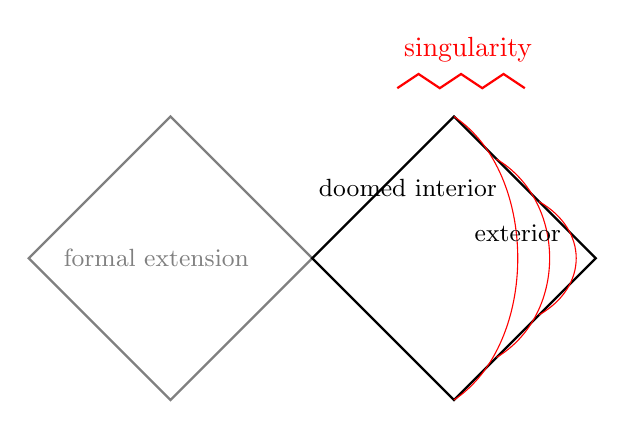
\begin{tikzpicture}[scale=0.9]
\draw[gray,thick] (-4,0) -- (-2,2) -- (0,0) -- (-2,-2) -- cycle;
\draw[thick] (0,0) -- (2,2) -- (4,0) -- (2,-2) -- cycle;

\draw[red,thick] (1.2,2.4) -- (1.5,2.6) -- (1.8,2.4) -- (2.1,2.6) -- (2.4,2.4) -- (2.7,2.6) -- (3.0,2.4);
\node[red] at (2.2,2.95) {singularity};

\draw[red] (2.0,-2.0) .. controls (3.2,-1.2) and (3.2,1.2) .. (2.0,2.0);
\draw[red] (2.6,-1.4) .. controls (3.6,-0.8) and (3.6,0.8) .. (2.6,1.4);
\draw[red] (3.2,-0.8) .. controls (3.9,-0.4) and (3.9,0.4) .. (3.2,0.8);

\node at (2.9,0.35) {\small exterior};
\node at (1.35,1.0) {\small doomed interior};
\node[gray] at (-2.2,0.0) {\small formal extension};
\end{tikzpicture}
\caption{Redibujo prudente del diagrama causal destacado en la clase: el exterior que se conserva, el interior condenado, la singularidad futura y el contraste con la parte formal adicional de la extensión.}
\end{figure}

En este punto, la clase es muy directa. Si estás en el exterior, aún puedes escapar o puedes caer dentro. Si estás en el interior, estás condenado. El diagrama ya muestra todo lo importante sobre el movimiento causal dirigido hacia el futuro.

Los cuadrantes \(III\) y \(IV\) son partes legítimas de la solución de Kruskal máximamente extendida. La región \(III\) proporciona un segundo exterior, y la región \(IV\) es la región de agujero negro con el tiempo invertido. Sin embargo, no aparecen en el espaciotiempo de un agujero negro ordinario formado por colapso. La solución extendida es instructiva desde el punto de vista matemático precisamente porque la construcción por colapso nos mostrará qué partes deben descartarse.

\section{Secciones espaciales, esferas bidimensionales y el puente de Einstein--Rosen}

Ahora fijemos el diagrama compactificado en una sección espacial y preguntémonos qué aspecto tiene esa sección como \emph{espacio}, en vez de como espaciotiempo. Aquí entra en escena la imagen del agujero de gusano, y es aquí donde no debemos dejar que la representación espacial se adelante al argumento causal.

Como se han suprimido las direcciones angulares, cada punto del diagrama radial representa una esfera bidimensional. A radio de Schwarzschild \(r\), su área es
\begin{equation}
A=4\pi r^2.
\end{equation}
Por tanto, una sección espacial es una familia de esferas bidimensionales, no simplemente una curva unidimensional. Su tamaño cambia al avanzar a lo largo de la sección.

Lejos del agujero, las esferas son muy grandes. Al avanzar hacia dentro, su radio disminuye hasta alcanzar un mínimo en el horizonte:
\begin{equation}
r_{\min}=2MG.
\end{equation}
Si se continúa a través de la extensión formal, las esferas vuelven a expandirse hacia otro lado asintótico. Esta es la imagen del puente de Einstein--Rosen.

\begin{figure}[htbp]
\centering
\includegraphics[width=0.72\textwidth]{lecture_08_figure_05.png}
\caption{Diagrama de Kruskal extendido con la sección espacial verde empleada para construir la geometría del puente. Cada punto de esa sección representa una esfera bidimensional; su radio mínimo está señalado en \(r=2MG\).}
\lectureframe{00:41:30}
\end{figure}

La pizarra muestra solo una parte del factor de Schwarzschild pertinente,
\begin{equation}
1-\frac{2MG}{r},
\end{equation}
y la garganta se encuentra en el mismo radio especial \(r=2MG\).

\begin{figure}[htbp]
\centering
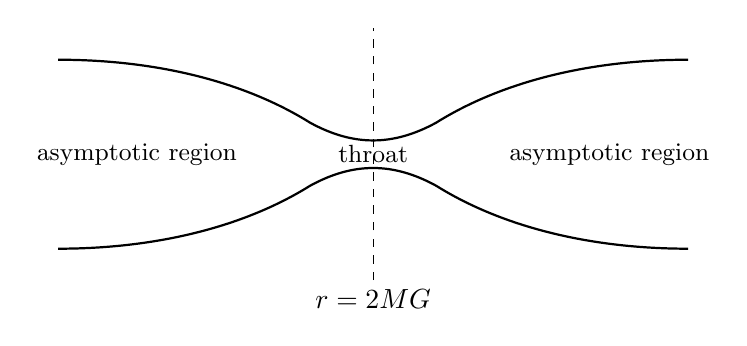
\begin{tikzpicture}[scale=1.0]
\draw[thick] (-4,1.2)
.. controls (-2.7,1.2) and (-1.6,0.9) .. (-0.8,0.4)
.. controls (-0.25,0.1) and (0.25,0.1) .. (0.8,0.4)
.. controls (1.6,0.9) and (2.7,1.2) .. (4,1.2);

\draw[thick] (-4,-1.2)
.. controls (-2.7,-1.2) and (-1.6,-0.9) .. (-0.8,-0.4)
.. controls (-0.25,-0.1) and (0.25,-0.1) .. (0.8,-0.4)
.. controls (1.6,-0.9) and (2.7,-1.2) .. (4,-1.2);

\draw[dashed] (0,-1.6) -- (0,1.6);
\node[below] at (0,-1.6) {$r=2MG$};
\node at (0,0) {\small throat};
\node at (-3.0,0) {\small asymptotic region};
\node at (3.0,0) {\small asymptotic region};
\end{tikzpicture}
\caption{Esquema de una sección espacial a través de la geometría de Schwarzschild extendida. Es una reconstrucción prudente de la imagen del puente presentada en la clase, no un cálculo literal de inmersión.}
\end{figure}

Ahora viene la corrección. La sección sugiere un puente entre dos regiones asintóticas e invita a pensar que quizá se podría viajar de un universo al otro atravesando el cuello. La clase deja que surja primero esa sugerencia y luego la descarta mediante un argumento causal. Para ir de una región exterior a la otra, una línea de universo tendría que ser, en algún punto del diagrama de Penrose, menos inclinada que una línea nula a \(45^\circ\). Eso está prohibido. Por tanto, el puente de Einstein--Rosen no es transitable.

El profesor también subraya por qué la representación espacial puede inducir a error. Es una representación del \emph{espacio en un instante de tiempo}, pero sencillamente no hay tiempo causal suficiente para atravesarlo. Puede decirse, de manera informal, que el puente se abre y se cierra antes de que algo pueda cruzarlo. Mejor aún, basta con volver al diagrama de Penrose y leer en él la respuesta causal.

\section{Construcción de un agujero negro real a partir de una capa nula entrante}

En este punto, la clase cambia por completo de problema. Ya no estamos deduciendo las propiedades de un agujero negro eterno. Vamos a construir uno real.

Se elige el modelo por su sencillez. Imaginamos no una estrella en colapso con una estructura interna complicada, sino una capa esférica delgada de radiación entrante. Es una capa de luz y, por tanto, se mueve hacia dentro a la velocidad de la luz. A un radio lo bastante pequeño, la energía de esa capa se concentra lo suficiente para que se forme un agujero negro.

El segundo ingrediente es el teorema de la capa en su formulación de relatividad general.

\paragraph{Observación.} Para la capa con simetría esférica considerada en esta clase, la región interior es un espaciotiempo plano y la región exterior es de Schwarzschild. Este es el teorema de la capa en su versión operativa, o enunciado de tipo Birkhoff, que emplea la clase. Aquí no se demuestra.

El profesor lo motiva recordando primero el teorema newtoniano de la capa: dentro de una capa esférica no hay campo gravitatorio, mientras que fuera de ella el campo es igual al de una masa puntual situada en el centro. Luego enuncia la versión relativista correspondiente en la única forma que necesitamos aquí: el interior es plano y el exterior es de Schwarzschild. La capa puede moverse; la regla sigue siendo la misma.

Con eso basta para construir el espaciotiempo del colapso. La propia capa es nula, así que debe dibujarse a \(45^\circ\). A un lado de esa línea nula, la geometría es plana. Al otro, es de Schwarzschild. Podemos resumir la regla así:
\begin{equation}
\begin{aligned}
\text{inside shell} &= \text{flat spacetime},\\
\text{outside shell} &= \text{Schwarzschild geometry}.
\end{aligned}
\end{equation}

La prescripción para unir las geometrías se vuelve entonces casi sorprendentemente sencilla:

\begin{enumerate}
\item Dibujar el diagrama de Penrose plano y conservar solo la región interior a la capa entrante.
\item Dibujar el diagrama de Penrose de Schwarzschild y conservar solo la región exterior a esa misma capa.
\item Descartar las partes que no corresponden.
\item Unir las dos partes conservadas a lo largo de la trayectoria de la capa.
\end{enumerate}

Así es exactamente como avanza la clase en la pizarra: descarta la mitad incorrecta de una representación, descarta la mitad incorrecta de la otra y une las mitades adecuadas a lo largo de la capa.

\begin{figure}[htbp]
\centering
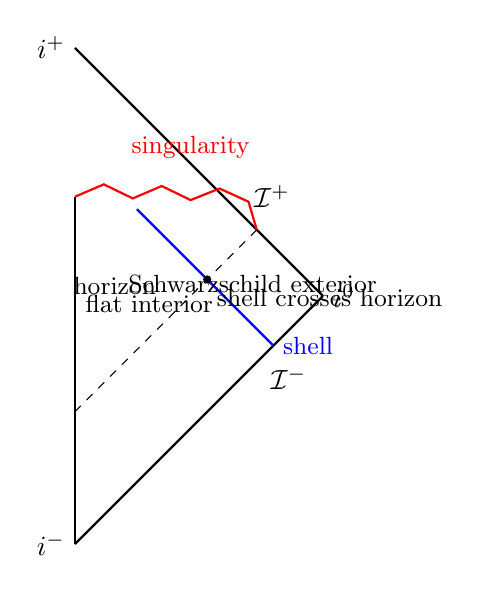
\begin{tikzpicture}[scale=1.05]
\coordinate (im) at (0,-3.0);
\coordinate (ip) at (0,3.0);
\coordinate (i0) at (3.0,0.0);
\coordinate (S)  at (0,1.2);
\coordinate (E)  at (2.2,0.8);
\coordinate (P)  at (2.4,-0.6);
\coordinate (Q)  at (0.75,1.05);
\coordinate (H)  at (0,-1.4);
\coordinate (X)  at (1.6,0.2);

\draw[thick] (im) -- (S);
\draw[thick] (im) -- (i0);
\draw[thick] (ip) -- (i0);

\draw[red,thick] (S) -- (0.35,1.35) -- (0.7,1.18) -- (1.05,1.33) -- (1.4,1.16) -- (1.75,1.30) -- (2.1,1.14) -- (E);
\node[red,above] at (1.4,1.55) {\small singularity};

\draw[thick,blue] (P) -- (Q);
\node[blue,right] at (P) {\small shell};

\draw[dashed] (H) -- (E);
\node[above left] at (1.1,-0.1) {\small horizon};

\filldraw (X) circle (1.2pt);
\node[below right] at (X) {\small shell crosses horizon};

\node at (0.9,-0.1) {\small flat interior};
\node at (2.15,0.15) {\small Schwarzschild exterior};

\node[left] at (im) {$i^-$};
\node[left] at (ip) {$i^+$};
\node[right] at (i0) {$i^0$};
\node[below right] at (2.25,-0.75) {$\mathcal{I}^-$};
\node[above right] at (2.05,0.95) {$\mathcal{I}^+$};
\end{tikzpicture}
\caption{Reconstrucción causal de la geometría del colapso. La capa es una línea nula entrante; se conserva el espaciotiempo plano en su lado interior y la geometría de Schwarzschild en su lado exterior.}
\end{figure}

\begin{figure}[htbp]
\centering
\includegraphics[width=0.76\textwidth]{lecture_08_figure_06.png}
\caption{Construcción final en la pizarra, después de unir el interior plano y el exterior de Schwarzschild a lo largo de la capa azul que cae hacia dentro. Se traza hacia atrás la línea discontinua \(45^\circ\) desde el extremo futuro de la singularidad para localizar el horizonte de sucesos.}
\lectureframe{00:57:30}
\end{figure}

La propia capa no experimenta nada especial cuando simplemente pasa de la parte plana del diagrama a la parte de Schwarzschild. Es una capa de tipo luz y continúa hacia dentro hasta llegar a la singularidad. La estructura esencial no depende de ningún suceso local espectacular en la capa, sino de la organización causal del espaciotiempo unido.

\begin{classroomqa}
\audiencequestion{¿Hay una discontinuidad cuando la capa en colapso atraviesa su radio de Schwarzschild?}
\lecturerresponse{No. En ese cruce no ocurre nada singular localmente. La capa continúa su trayectoria nula. El suceso especial es de carácter causal: después de que la capa haya atravesado su propio radio \(2MG\), ningún camino dirigido hacia el futuro puede llevarla de vuelta al infinito.
\lecturetimestamp{00:56:19--00:56:42}}
\end{classroomqa}

\section{El horizonte antes de la llegada: el enigma del horizonte de sucesos}

Ahora llega el clímax conceptual de la clase. Una vez construido el espaciotiempo del colapso, la pregunta natural es: ¿dónde está el horizonte? O, como dice el profesor, ¿dónde está el punto de no retorno?

\paragraph{Definición.} El horizonte de sucesos es la frontera entre los sucesos que aún pueden enviar una señal causal dirigida hacia el futuro a \(\mathcal{I}^+\) y aquellos que no pueden hacerlo.

La clase lo localiza en el diagrama. Partimos del vértice donde la singularidad se encuentra con el infinito nulo futuro y trazamos hacia atrás una línea nula a \(45^\circ\). Esa línea nula trazada hacia atrás es el horizonte de sucesos.

Pero el profesor insiste luego en un segundo punto, que es el que inquieta a los estudiantes. El horizonte no aparece simplemente en el momento en que la capa atraviesa su propio radio de Schwarzschild para luego quedarse allí. En el dibujo ampliado de la pizarra, el horizonte comienza como una pequeña región atrapada cerca del centro, se expande hacia fuera por una parte del espaciotiempo que todavía es plana y solo más tarde se encuentra con la capa entrante. En el suceso de ese encuentro, la capa atraviesa su propio radio de Schwarzschild. Por encima de ese suceso, el horizonte es el horizonte ordinario de radio constante del agujero negro ya formado.

\begin{figure}[htbp]
\centering
\resizebox{0.96\linewidth}{!}{%
\begin{tikzpicture}[scale=1.08,>=Latex]
\coordinate (im) at (0,-3.0);
\coordinate (ip) at (0,3.0);
\coordinate (i0) at (3.0,0.0);
\coordinate (S)  at (0,1.2);
\coordinate (E)  at (2.2,0.8);
\coordinate (P)  at (2.4,-0.6);
\coordinate (Q)  at (0.75,1.05);
\coordinate (H)  at (0,-1.4);
\coordinate (X)  at (1.6,0.2);

\draw[thick] (im) -- (S);
\draw[thick] (im) -- (i0);
\draw[thick] (ip) -- (i0);

\draw[red,thick] (S) -- (0.35,1.35) -- (0.7,1.18) -- (1.05,1.33) -- (1.4,1.16) -- (1.75,1.30) -- (2.1,1.14) -- (E);
\node[red,above left] at (S) {\small singularity};

\draw[very thick,red] (H) -- (E);

\draw[thick,blue] (P) -- (Q);

\filldraw (X) circle (1.2pt);

\draw[gray] (0.0,-2.1) .. controls (0.85,-1.95) and (1.9,-1.3) .. (2.8,-0.2);
\draw[gray] (0.0,-1.2) .. controls (0.95,-1.0) and (1.8,-0.45) .. (2.45,0.35);
\draw[gray] (0.0,-0.2) .. controls (0.8,-0.05) and (1.45,0.35) .. (1.95,0.95);

\node[below right] at (2.28,-0.72) {$\mathcal{I}^-$};
\node[above right] at (2.12,0.92) {$\mathcal{I}^+$};

\draw[very thick,red] (3.2,-1.15) -- (3.75,-1.15);
\node[anchor=west] at (3.85,-1.15) {\small event horizon};
\draw[thick,blue] (3.2,-1.55) -- (3.75,-1.55);
\node[anchor=west] at (3.85,-1.55) {\small infalling shell};
\filldraw (3.48,-1.95) circle (1.2pt);
\node[anchor=west] at (3.85,-1.95)
  {\small shell reaches \(r=2MG\)};
\end{tikzpicture}
}
\caption{Diagrama del colapso en el que se destaca el horizonte de sucesos trazado hacia atrás. Una parte del horizonte se encuentra en una región que aún es localmente plana y a la que la capa todavía no ha llegado.}
\end{figure}

Este es el efecto sorprendente en el que se detiene el resto de la clase. Parte del horizonte está en el espaciotiempo plano. La capa aún no ha llegado allí, y ni siquiera es visible en el cono de luz pasado del observador. El observador no siente ningún campo gravitatorio y, sin embargo, no puede escapar. La razón no es una fuerza local, sino el futuro causal global del suceso.

\begin{classroomqa}
\audiencequestion{¿La construcción dice que no se puede atravesar la capa o que no se puede atravesar el horizonte? ¿Dónde está la capa cuando su horizonte todavía queda por dentro de ella?}
\lecturerresponse{Se puede atravesar la capa. El horizonte es otra superficie nula: la frontera entre los sucesos que pueden comunicarse con \(\mathcal I^+\) y los que no. La capa entrante se encuentra con esa frontera justo cuando atraviesa el radio de Schwarzschild asociado a su energía total. Antes de ese encuentro, parte del horizonte de sucesos atraviesa el interior plano; después, la capa queda dentro del agujero negro ya formado.
\lecturetimestamp{00:58:42--01:01:06}}
\end{classroomqa}

\begin{classroomqa}
\audiencequestion{Si el interior es plano y la capa todavía está lejos, ¿por qué alguien que está justo dentro del horizonte no puede cruzarlo antes de que llegue la capa?}
\lecturerresponse{Trace la línea de universo saliente más rápida posible: un rayo de luz de \(45^\circ\). Desde un suceso situado dentro del horizonte trazado hacia el pasado, incluso ese rayo alcanza la capa entrante demasiado tarde y termina en la singularidad. Caminar es aún más lento. La frase \emph{la capa aún no ha cruzado} queda incompleta mientras no se elija una coordenada temporal; el diagrama causal da la respuesta independiente de las coordenadas. La radiación cósmica de fondo entrante no es el mismo ejemplo, porque no es una capa esférica en colapso que cree esta geometría.
\lecturetimestamp{01:01:07--01:04:03}}
\end{classroomqa}

\section{Espejos e intentos de cambiar el futuro}

Las preguntas convierten ahora el diagrama en un laboratorio. Supongamos que se pudiera reflejar una capa de luz entrante antes de que quedara atrapada. Entonces cambiaría la historia de colapso supuesta y también el horizonte de sucesos. No hay contradicción: el horizonte de sucesos solo queda definido una vez especificada la historia completa del espaciotiempo.

\begin{classroomqa}
\audiencequestion{¿Qué ocurriría si se colocara un espejo perfectamente reflectante justo fuera del radio de Schwarzschild que se alcanzaría, de modo que la capa rebotara hacia fuera?}
\lecturerresponse{En esa historia idealizada, la línea nula entrante cambia de sentido en el espejo y llega a la frontera futura; el agujero negro del diagrama original no se forma. Un espejo verdaderamente ingrávido es imposible, y un espejo físico aporta su propio tensor de energía-momento, pero el experimento mental deja claro el argumento lógico: solo después de que la capa atraviese el horizonte de sucesos real deja de ser posible escapar.
\lecturetimestamp{01:04:33--01:05:54}}
\end{classroomqa}

\begin{classroomqa}
\audiencequestion{¿Podría un observador que sabe que la capa se acerca enviar rápidamente un espejo o una señal para hacer que dé la vuelta?}
\lecturerresponse{Solo si el dispositivo necesario puede colocarse fuera del horizonte con suficiente antelación. Alice puede acordar de antemano que Bob envíe la capa y, por tanto, saber lo que se acerca antes de verla. Sin embargo, una vez que su suceso está dentro del horizonte, ni un espejo ni una instrucción pueden llegar a tiempo al punto exterior necesario. Conocer de antemano el experimento futuro no abre un camino causal que el diagrama prohíbe.
\lecturetimestamp{01:05:55--01:08:18}}
\end{classroomqa}

\begin{classroomqa}
\audiencequestion{¿Qué le ocurre a un espejo que ya está dentro del horizonte, y la singularidad está infinitamente lejos en su futuro?}
\lecturerresponse{El espejo es simplemente otro objeto condenado. Puede reflejar la luz localmente, pero la luz reflejada, el espejo y Alice terminan en la singularidad. Una línea de universo genérica de un objeto en caída la alcanza en un tiempo propio finito. Solo el vértice superior ideal del diagrama compactificado está infinitamente lejos. Intentar permanecer cerca de ese vértice exigiría una aceleración y una energía ilimitadas; además, entre sucesos fijos, un reloj acelerado acumula menos tiempo propio que uno inercial, no más.
\lecturetimestamp{01:08:19--01:10:19}}
\end{classroomqa}

\begin{classroomqa}
\audiencequestion{Si la capa en colapso es enorme, ¿puede alguien que esté dentro de ella, pero lejos de su centro futuro, quedarse allí mientras pasa?}
\lecturerresponse{Sí, siempre que el suceso de esa persona siga estando fuera del horizonte de sucesos. Estar dentro de la capa material no es lo mismo que estar dentro del agujero negro. La radiación puede alcanzar y herir al observador, pero eso es una interacción local con la capa, independiente de la cuestión causal de si puede escapar.
\lecturetimestamp{01:10:21--01:11:24}}
\end{classroomqa}

\section{Secciones temporales y crecimiento del horizonte}

Un \emph{instante de tiempo} en el espacio-tiempo curvo significa una hipersuperficie espacial elegida. Una sucesión de esas superficies constituye una foliación, y asignar un número a cada superficie define una coordenada temporal. Distintas foliaciones cortan de manera diferente el mismo diagrama del colapso. Difieren en qué sucesos distantes son simultáneos, pero no cambian qué rayos nulos llegan al infinito.

\begin{figure}[htbp]
\centering
\includegraphics[width=0.77\textwidth]{lecture_08_figure_07.png}
\caption{El diagrama tardío en la pizarra, con varias secciones espaciales verdes. Las secciones proporcionan una coordenada temporal; las fronteras nulas negras y sus relaciones causales son independientes de esa elección.}
\lectureframe{01:17:30}
\end{figure}

\begin{classroomqa}
\audiencequestion{¿Puede reformularse el problema comparando, en un mismo instante, la distancia del observador al horizonte con la distancia del horizonte a la capa?}
\lecturerresponse{Puede ser una intuición útil una vez elegida una foliación, pero la expresión \emph{en un mismo instante} depende de las coordenadas. La construcción más clara consiste en dibujar una familia de secciones espaciales. Las secciones tempranas atraviesan una capa grande y ninguna región central atrapada; las posteriores atraviesan el horizonte creciente dentro de la capa que aún está cayendo; una sección particular pasa por el suceso en que la capa cruza su propio radio de Schwarzschild.
\lecturetimestamp{01:11:26--01:14:21}}
\end{classroomqa}

\begin{classroomqa}
\audiencequestion{¿Crece el radio de Schwarzschild a medida que el horizonte se extiende hacia afuera, y por qué sigue creciendo el horizonte después de que la capa lo cruza?}
\lecturerresponse{El radio de Schwarzschild final \(2MG\) es fijo porque la masa total \(M\) es fija. Lo que crece en las secciones espaciales tempranas es el radio areal de la sección transversal del horizonte. Empieza en el centro, aumenta hasta encontrarse con la capa en \(r=2MG\) y luego deja de crecer. Por encima del suceso de encuentro, el horizonte es la línea constante \(r\) \(r=2MG\), aunque la compactificación no haga que esa línea parezca vertical ni uniforme en términos métricos.
\lecturetimestamp{01:14:22--01:16:15}}
\end{classroomqa}

\begin{classroomqa}
\audiencequestion{¿Qué le ocurre a un observador que inicialmente está a la mitad del radio de Schwarzschild final? ¿No debería ese observador sentir la gravedad solo cuando llega la capa?}
\lecturerresponse{Exactamente. El observador cruza primero el horizonte de sucesos creciente mientras todavía está en el espacio-tiempo plano, y no siente ninguna fuerza repentina. Más tarde puede sentir la capa de radiación que cae, pues es material; el horizonte de sucesos, en cambio, no lo es. Cruzarlo solo significa que, a partir de entonces, ninguna trayectoria causal dirigida hacia el futuro puede llegar al infinito. En ese sentido preciso, el horizonte es fantasmal.
\lecturetimestamp{01:16:17--01:17:45}}
\end{classroomqa}

\begin{classroomqa}
\audiencequestion{¿Puede un observador que parte con suficiente antelación desplazarse hacia afuera más rápido que el horizonte creciente y escapar?}
\lecturerresponse{Los sucesos exteriores al horizonte tienen trayectorias causales salientes hacia \(\mathcal I^+\); los interiores, no. En una sección elegida se puede comparar la distancia radial disponible con el tiempo que falta para que la capa entrante cierre la ruta, pero las líneas nulas ofrecen la prueba exacta. Ningún observador ve un horizonte material precipitándose hacia afuera, porque no hay una superficie local que pueda verse.
\lecturetimestamp{01:17:46--01:18:54}}
\end{classroomqa}

\section{Qué conserva el diagrama}

Las formas de la página no deben interpretarse como un dibujo a escala. Una esquina pequeña puede representar una región infinita del espacio-tiempo, mientras que una zona amplia puede representar un intervalo físico modesto. La compactificación sacrifica deliberadamente el tamaño métrico para conservar las direcciones nulas. Lo que se conserva es la causa y el efecto: quién puede enviar una señal a quién, qué sucesos pueden influir en cuáles y qué líneas de universo quedan atrapadas por el límite de la velocidad de la luz.

\begin{classroomqa}
\audiencequestion{Si la imagen distorsiona tanto las longitudes y los tiempos, ¿qué representa fielmente?}
\lecturerresponse{Representa los rayos de luz y, por tanto, la estructura causal. Para localizar el horizonte de sucesos, hay que trazar hacia atrás desde el infinito futuro el último rayo nulo saliente. No es fiable intentar deducir la respuesta a partir de las distancias aparentes en la página. Una vez dibujado el diagrama causal, las preguntas sobre señales, escape y la imposibilidad de regresar tienen respuestas geométricas, aunque se haya omitido la escala métrica.
\lecturetimestamp{01:18:56--01:21:45}}
\end{classroomqa}

\begin{classroomqa}
\audiencequestion{¿Cuánto se tarda en sentirse lo bastante cómodo con los diagramas de Penrose como para usarlos intuitivamente?}
\lecturerresponse{No mucho. El método práctico consiste en dibujarlos, trazar líneas nulas y examinar posibles líneas de universo hasta familiarizarse con las restricciones causales. La intuición se adquiere trabajando con los diagramas, no haciendo conjeturas sin ellos.
\lecturetimestamp{01:21:49--01:22:05}}
\end{classroomqa}

\begin{classroomqa}
\audiencequestion{¿Es este método visual lo opuesto a la mecánica cuántica, donde las matemáticas suelen ser más fiables que una imagen?}
\lecturerresponse{En buena medida, sí. La relatividad general es física clásica. Es difícil imaginar literalmente el espacio-tiempo curvo de cuatro dimensiones, y un diagrama de Penrose sigue siendo abstracto, pero su geometría causal puede dibujarse y explorarse mucho más a fondo de lo que puede hacerse con la realidad subyacente de la mecánica cuántica. Esa diferencia es parte de lo que hace tan poderosos estos diagramas.
\lecturetimestamp{01:22:05--01:22:58}}
\end{classroomqa}